\documentclass[a4paper]{scrartcl}
\usepackage[cm]{fullpage}
\usepackage{amsmath, amssymb}

\usepackage{sectsty}
\sectionfont{\large\selectfont}
\subsectionfont{\normalsize\selectfont}

\usepackage{siunitx}
\usepackage{tikz}

\begin{document}

\title{PHYS1241: Assignment 2}
\author{ \\ \\ }
\date{2015-09-08}
\maketitle

\section{In a certain region of space, there is a uniform electric field \(\mathbf{E}\) of \SI{10000}{\volt\per\centi\metre} in the \(+x\) direction. In the same region of space there is a uniform magnetic field \(\mathbf{B}\) in the \(+y\) direction. A beam of mu-mesons with velocity \(\frac{c}{3}\) travels through this region in a straight line in the \(+z\) direction.}
\subsection{What is the strength of the field \(\mathbf{B}\)?}
Since the charges are travelling in a straight line with constant velocity, there must be no net force acting on them, and this can be used to calculate the magnetic field:
\begin{align*}
    \mathbf{E} &= \begin{pmatrix}\mathbf{E}_x \\ 0 \\ 0\end{pmatrix},
    \mathbf{B} = \begin{pmatrix}0 \\ \mathbf{B}_y \\ 0\end{pmatrix},
    \mathbf{v} = \begin{pmatrix}0 \\ 0 \\ \mathbf{v}_z\end{pmatrix} \\
    \mathbf{F} &= q (\mathbf{E} + \mathbf{v} \times \mathbf{B}) = \mathbf{0} \\
    &= q \begin{pmatrix}\mathbf{E}_x - \mathbf{v}_z \mathbf{B}_y \\ 0 \\ 0\end{pmatrix} \\
    \therefore \mathbf{E}_x &= \mathbf{v}_z \mathbf{B}_y \\
    \mathbf{B}_y &= |\mathbf{B}| = \frac{\mathbf{E}_x}{\mathbf{v}_z} \\
    &= \frac{\SI{30000}{\volt\per\centi\metre}}{c} \approx \SI{10}{\milli\tesla}
\end{align*}

\subsection{Can you tell from this experiment if the charge on the meson is positive or negative?}
No, since the \(q\) term in the equation turns out to be irrelevant.

Physically, a positive charge would be attracted to the \(+x\) direction by the \(\mathbf{E}\)-field, and to the \(-x\) direction by the \(\mathbf{B}\)-field, and the exact opposite would happen for a negative charge. But since the charge travels in a straight line, that is, experiencing no net force, the two fields balance each other perfectly so it is impossible to determine whether the charge is attracted to \(+x\) or \(-x\) by the \(\mathbf{E}\)- or \(\mathbf{B}\)-field, and thus impossible to determine the sign of the charge.

\section{A metal spherical shell of inner radius \(a\) and outer radius \(b\) is located with its centre at the origin. There is a small hole cut at one point of the shell.}
\subsection{If there is no net charge on the shell, how much work is required to bring a charge \(q_1\) from infinity, through the hole and to the origin?}
No work is required, as the uncharged shell does not generate any electric potential.

\subsection{How much work is required if the shell is given a total charge \(q_2\)?}
Find the electric potential at the centre of the charged shell, and then multiply it by \(q_1\) to determine the work required. Since a charged conductor will have the charges distributed only over its outer surface, we only need to consider the sphere as if it were a infinitesimally thin sphere at \(r = b\).
\begin{align*}
    V_E &= \iint_S \frac{\mathrm{d}q_2}{4 \pi \varepsilon_0 r} \\
    &= \int_0^\pi \int_0^{2 \pi} \frac{\sigma}{4 \pi \varepsilon_0 r} r^2 \sin \phi \,\mathrm{d}\theta \,\mathrm{d}\phi \\
    \sigma &= \frac{q_2}{4 \pi r^2} \\
    V_E &= \frac{q_2}{(4 \pi)^2 \varepsilon_0 r} \int_0^\pi \int_0^{2 \pi} \sin \phi \,\mathrm{d}\theta \,\mathrm{d}\phi \\
    &= \frac{q_2}{4 \pi \varepsilon_0 r} \\
    \therefore U_E \bigg|_{r = b} &= q_1 V_E \bigg|_{r = b} \\
    &= \frac{q_1 q_2}{4 \pi \varepsilon_0 b}
\end{align*}

\section{A parallel plate capacitor is connected to a battery that maintains a potential difference \(V_0\) between its plates. A slab of dielectric constant \(\kappa\) is inserted between the plates, completely filling the space between them.}
\subsection{Show that the battery does an amount of work \(q_0 V_0 (\kappa - 1)\) during the insertion process, if \(q_0\) is the charge on the capacitor before the slab is inserted.}

\subsection{How much work is done by mechanical forces on the slab when it is inserted between the plates? Is this work done on, or by, the agent inserting the slab?}

\section{A wire bent is into the shape shown. A current \(I = \SI{15}{\ampere}\) flows through the wire, \(a\) has length \SI{5.2}{\centi\metre}. What is the magnetic field \(\mathbf{B_P}\) at point \(P\)?}
\begin{center}
    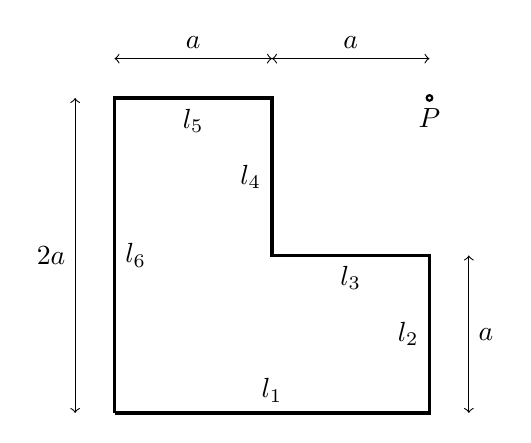
\begin{tikzpicture}
        \draw [very thick]
            (0, 0) -- (4, 0) node[midway, above] {\(l_1\)}
            -- (4, 2) node[midway, left] {\(l_2\)}
            -- (2, 2) node[midway, below] {\(l_3\)}
            -- (2, 4) node[midway, left] {\(l_4\)}
            -- (0, 4) node[midway, below] {\(l_5\)}
            -- (0, 0) node[midway, right] {\(l_6\)};
        \draw [thick] (4, 4) circle (1 pt) node [below] {\(P\)};
        \draw [<->] (-0.5, 0) -- (-0.5, 4) node [midway, left] {\(2 a\)};
        \draw [<->] (0, 4.5) -- (2, 4.5) node [midway, above] {\(a\)};
        \draw [<->] (2, 4.5) -- (4, 4.5) node [midway, above] {\(a\)};
        \draw [<->] (4.5, 2) -- (4.5, 0) node [midway, right] {\(a\)};
    \end{tikzpicture}
\end{center}
We can use the Biot-Savart law to find the magnetic field due to a wire segment, and then apply it to each segment of the wire loop.

For a wire segment on the \(+x\) axis starting at the origin and of length \(l\), and constant current \(I\) flowing away from the origin, the magnetic field can be derived for any arbitrary 2D displacement:
\begin{align*}
    \mathbf{B}(\mathbf{r}) &= \frac{\mu_0 I}{4 \pi} \int_C \frac{\mathrm{d}\mathbf{l} \times \mathbf{r}'}{|\mathbf{r}'|^3} \\
    \mathbf{r} &= \begin{pmatrix}x \\ y \\ 0\end{pmatrix}, \mathbf{l} = \begin{pmatrix}l \\ 0 \\ 0\end{pmatrix} \\
    \mathbf{r}' &= \mathbf{r} - \mathbf{l} = \begin{pmatrix}x - l \\ y \\ 0\end{pmatrix} \\
    \mathrm{d}\mathbf{l} \times \mathbf{r}' &= \begin{pmatrix}0 \\ 0 \\ y \,\mathrm{d}l\end{pmatrix} \\
    \therefore \mathbf{B}(\mathbf{r}) &= \frac{\mu_0 I}{4 \pi} \begin{pmatrix}
        0 \\ 0 \\
        \int_0^l \frac{y \,\mathrm{d}l}{((x - l)^2 + y^2)^{\frac{3}{2}}}
    \end{pmatrix} \\
    \therefore \mathbf{B}_z(\mathbf{r}) &= \begin{cases}
        0 & y = 0 \\
        \frac{\mu_0 I}{4 \pi y} \left( \frac{l - x}{\sqrt{(l - x)^2 + y^2}} + \frac{x}{\sqrt{x^2 + y^2}} \right) & \text{Otherwise}
    \end{cases}
\end{align*}

Now consider going anticlockwise around the wire loop starting at wire segment \(l_1\), placing the origin of each wire segment at the start of each and the \(+x\) axis along the wire. This can be done because \(\mathbf{B}(\mathbf{r})\) is independent of the \(x\) and \(y\) axis. \(\mathbf{B_P}\) can then be calculated:
\begin{align*}
    \mathbf{B_P}_z &=
    \mathbf{B}_z\begin{pmatrix}2 a \\ 2 a \\ 0\end{pmatrix} \bigg|_{l = 2 a} +
    \mathbf{B}_z\begin{pmatrix}2 a \\ 0 \\ 0\end{pmatrix} \bigg|_{l = a} +
    \mathbf{B}_z\begin{pmatrix}0 \\ -a \\ 0\end{pmatrix} \bigg|_{l = a} \\
    &+ \mathbf{B}_z\begin{pmatrix}a \\ -a \\ 0\end{pmatrix} \bigg|_{l = a} +
    \mathbf{B}_z\begin{pmatrix}-a \\ 0 \\ 0\end{pmatrix} \bigg|_{l = a} +
    \mathbf{B}_z\begin{pmatrix}0 \\ 2 a \\ 0\end{pmatrix} \bigg|_{l = 2 a} \\
    &= \frac{-\mu_0 I}{4 \pi a \sqrt{2}} \\
    \therefore \mathbf{B_P} &= \begin{pmatrix}0 \\ 0 \\ \frac{-\mu_0 I}{4 \pi a \sqrt{2}}\end{pmatrix} \approx \begin{pmatrix}0 \\ 0 \\ -20\end{pmatrix}\si{\micro\tesla}
\end{align*}
Where \(I\) is assumed to be flowing anticlockwise. If it were flowing clockwise, the sign would just be reversed. In other words, an anticlockwise current would cause \(\mathbf{B_P}\) to be in to the page, while a clockwise would be out of the page.

\section{A very long conducting rod of radius \(a\) has an off-centre hole of radius \(b\) whose axis is parallel to but offset by a distance \(d\) from the axis of the rod. A uniform current density \(+j\) flows in the conductor. What is the magnetic field \(\mathbf{B}\) at the axis of the hole, far from the ends?}

\section{Consider two coaxial loops of radius \(a\) which are separated by a distance \(d; d \gg a\). A current \(I = K_0 t^2\) is sent through loop (1). The resistance of the other loop is \(R\).}
\subsection{Neglecting self-inductance, what is the torque, \(\tau\), on loop (2)?}

\subsection{Show that, if the self inductance is neglected, the force on loop (2) is \(K = \frac{24 \pi^4 a^8 K_0^2 t^3}{(4 \pi \varepsilon_0 c^2)^2 d^7 R}\).}

\subsection{In what direction is the force?}

\subsection{In what way (quantitatively) is the true force and torque different from your estimate; i.e., how does self-inductance affect the torque and force?}

\subsection{Explain what happens in part (a) and (b) above if loop (2) were rotated \SI{90}{\degree} about an axis normal to the common axis of the loops.}

\end{document}
